\documentclass{standalone}
\usepackage{tikz}
\usetikzlibrary{matrix}
\begin{document}
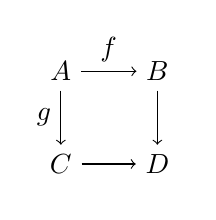
\begin{tikzpicture}
\matrix (m) [matrix of math nodes, row sep=2em, column sep=2em]
{ A & B \\ C & D \\ };
\draw[->] (m-1-1) -- node[above] {$f$} (m-1-2);
\draw[->] (m-1-1) -- node[left] {$g$} (m-2-1);
\draw[->] (m-2-1) -- (m-2-2);
\draw[->] (m-1-2) -- (m-2-2);
\end{tikzpicture}
\end{document}
